\documentclass[]{algotel}

\usepackage[latin1]{inputenc}
\usepackage[francais]{babel}
\usepackage{tikz}
\usepackage{amsmath,accents}
\usepackage{amsthm}
\usepackage{subcaption}
\captionsetup{compatibility=false}
\usepackage{amsfonts}
\usepackage{wrapfig}
\usepackage[noabbrev,capitalize]{cleveref}
\usepackage[]{mdframed}
\newtheorem{theorem}{Theorem}
\newtheorem{lemma}{Lemma}
\newtheorem{fact}{Fact}
\newtheorem{corollary}{Corollary}
\newtheorem{definition}{Definition}
\newtheorem{conjecture}{Open question}


\author{Arnaud Casteigts\addressmark{1}
	\and
	Mathieu Raffinot\addressmark{1}
	\and
	Jason Schoeters\addressmark{1}}

\title[VectorTSP : un probl�me de voyageur de commerce avec des contraintes d'acc�l�ration]{\textsc{VectorTSP} : un probl�me de voyageur de commerce avec des contraintes d'acc�l�ration\footnote{La version anglaise de ce travail a �t� publi�e � ALGOSENSORS 2020~\cite{casteigts2020vectortsp}.\\ Ce travail a �t� soutenu par le projet ANR ESTATE (ANR-16-CE25-0009-03).}}

\address{\addressmark{1}Univ. Bordeaux, Bordeaux INP, CNRS, LaBRI, UMR5800, F-33400 Talence, France}


\keywords{voyageur de commerce, planification de mouvements, contraintes d'acc�l�ration, probl�me d'optimization}

\begin{document}
\maketitle

\begin{abstract}
	Nous nous int�ressons � une nouvelle version du \textsc{TSP} Euclidien, appel�e \mbox{\textsc{VectorTSP}} (ou \textsc{VTSP}) dans laquelle une entit� mobile peut se d�placer par rapport � un ensemble de contraintes physiques inspir�es du jeu de papier et crayon \textsc{Racetrack} (aussi appel� \textsc{Vector Racer}). Compar�e � d'autres versions du \textsc{TSP} avec contraintes physiques, comme le \textsc{Dubins TSP}, l'esprit de ce mod�le est que (1) il n'y a pas de limitations de vitesse, et (2) l'inertie d�pend de la vitesse actuelle. Ce mod�le est donc plus proche des mod�les typiquement consid�r�s dans des probl�mes de planification de mouvements, et est ici appliqu� � la visite de $n$ villes dans un ordre non-pred�termin�. Nous pr�sentons ce probl�me en discutant des diff�rences fondamentales avec d'autres versions de \textsc{TSP}. En particulier, un ordre de visite optimal pour \textsc{ETSP} peut ne pas �tre optimal pour \textsc{VTSP}. Nous d�montrons que \mbox{\textsc{VectorTSP}} est $NP$-difficile, et dans l'autre sens, que \textsc{VectorTSP} se r�duit vers \textsc{GroupTSP} en temps polynomial.
	D'un point de vue algorithmique, nous proposons un sch�ma interactif entre un algorithme haut niveau et un oracle de trajectoire. Le premier permet de calculer l'ordre de visite, tandis que le second calcule le co�t (ou la trajectoire) pour un ordre de visite donn�.
	Nous pr�sentons des algorithmes pour les deux, et nous d�montrons et quantifions exp�rimentalement que cette approche trouve souvent une meilleure solution que la trajectoire optimale r�sultant d'un ordre de visite optimal \textsc{ETSP}. 
\end{abstract}

\section{Introduction}

%TSP

The problem of visiting a given set of places and returning to the starting point, while minimizing the total cost, is known as the Traveling Salesperson Problem (TSP, for short).
%The problem was independently formulated by Hamilton and Kirkman in the 1800s and has been extensively studied since.
%Many versions of this problem exist, motivated by applications in various areas, such as vehicle routing, computer wiring, stock cutting, and DNA reconstruction.
An instance of the problem can be given as a graph whose vertices represent the places to visit (often referred to as {\em cities}) and weights on the edges represent the cost of moving from one city to another. 
%The decision version thenOne is asked to find the minimum cost tour (optimization version) or to decide whether a tour having at most some cost exists (decision version) subject to the constraint that every city is visited {\em exactly} once.
Karp proved in 1972 that the \textsc{Hamiltonian Cycle} problem is $NP$-hard, which implies that \textsc{TSP} is $NP$-hard~\cite{karp1972reducibility}.
TSP was subsequently shown to be inapproximable (unless $P = NP$) by Orponen and Manilla in 1990~\cite{orponenmannila90}. On the positive side, while the trivial algorithm has a factorial running time (essentially, evaluating all permutations of the visit order), Held and Karp presented % 1962
a dynamic programming algorithm~\cite{heldkarp62} running in time $O(n^22^n)$, which as of today remains the fastest known exact algorithm.
% WILLDO is Held-Karp optimal under ETH? It seems that no such results were proven yet.

Many special cases of \textsc{TSP} are considered in the literature, motivated by applications in various areas, such as vehicle routing, computer wiring, stock cutting, and DNA reconstruction. We will go over the most relevant ones \textit{w.r.t.} this paper.
%In Symmetric TSP, on has $cost(u,v) = cost(v,u)$ for all cities $u,v$.
%In Metric TSP (a subclass of Symmetric TSP), the costs respect the triangle inequality, namely $cost(u,v) \le cost(u,w) + cost(w,v)$ for all cities $u,v,w$.
%, and the constraint of visiting a city exactly once is relaxed (or equivalently, it is not, but the instance is turned into a complete graph where the weight of every edge $uv$ is the cost of a shortest \emph{path} from $u$ to $v$ in the original instance).
%\textsc{Metric TSP} was shown to be approximable within factor $1.5$ by Christofides~\cite{christofides76}. Whether the factor is optimal is unknown, although it cannot be less than $1.0045$ (unless $P = NP$) and so no PTAS exists for Metric TSP~\cite{PV06}. Asymmetric TSP in which the triangle inequality holds can be approximated to a factor of $22 + \epsilon$~\cite{traub2020improved}, for any $\epsilon > 0$.
In \textsc{Euclidean TSP} (\textsc{ETSP}, for short), the cities are points in the plane, and weights are the Euclidean distance between cities. 
%This version is known as the Euclidean TSP (ETSP, for short). 
This problem, although still $NP$-hard (proven by Papadimitriou~\cite{papadimitriou1977euclidean} and Garey \textit{et al.}~\cite{garey1976some}), was shown to admit a polynomial-time approximation scheme (PTAS) by Arora~\cite{arora96} and Mitchell~\cite{mitchell99}.
\textsc{Dubins TSP} (\textsc{DTSP}), which is also $NP$-hard (proven by Le Ny \textit{et al.}~\cite{le2007curvature}), accounts for inertia by bounding the curvature of a trajectory by a fixed radius. This may represent for example a vehicle with wheels of bounded turning angles, such as cars.
%This approach offers an elegant (\textit{i.e.} purely geometrical) abstraction to the problem. 
Savla \textit{et al.}~\cite{savla2009traveling} introduce the \textsc{Double Integrator TSP}, which considers a continuous-time model of acceleration for the visiting vehicle, and give some probabilistic results on the stochastic version of the problem. 

The aim of this paper is to introduce and study a version of \textsc{TSP} which may accurately represent a visiting vehicle with acceleration, \textit{i.e.} which can use sharp turns at low speed, but experiences inertia forces at high speeds. In contrast to Savla \textit{et al.}'s continuous model (see~\cite{savla2009traveling}) which is more related to control theory, we focus on a discrete model of acceleration which is naturally prone to algorithmic investigation.

% accounts for speed variations; for example, it does not enable sharper turns when the speed is low, nor does it account for inertia beyond a fixed speed.
%More realistic models have been considered beyond TSP, such as in the context of the path planning problem, where one aims to find an optimal trajectory between two given points (with obstacles), while satisfying constraints on acceleration/inertia. More generally, the literature on {\it kinodynamics} is vast (see, e.g.~\cite{canny1988complexity,canny1991exact,donald1993kinodynamic} for some relevant examples). The constraints are often formulated in terms of the considered space's dimensions, a bounded acceleration and a bounded speed. The positions may either be considered in a discrete domain or continuous domain, the latter being more related to the fields of control theory and analytic functions. In constrast, the discrete domain is naturally prone to algorithmic investigation. 

%RACETRACK

In a recreative column of the {\em Scientific American} in 1973~\cite{gardner1973sim}, Martin Gardner presented a paper-and-pencil game known as \textsc{Racetrack} (as well as Vector Racer, Graph Racer, Vector Rally, \textit{etc.}).
The game is played by each player controlling its respective vehicle's speed, which, each round, may be modified in a simple and discrete manner.  
%Other names for this game include Vector Racer, Graph Racer, Vector Rally, Vector Race, Vektorrennen (in German) and Le Zip (in French).
%The game is played in \textbf{rounds}, by multiple players, in which they compete to finish first. 
The game is in fact a motion planning optimization problem, with the natural parameter to minimize being the amount of rounds needed for a mobile entity to arrive at the finish area.
In \cite{holzer2010computational}, Holzer \textit{et al.} show \textsc{Racetrack} is in $NL$, and verifying if a given strategy for Racetrack is winning is $P$-hard which contradicts the popular ``conjecture'' stating that all interesting and fun games are $NP$-hard.
In \cite{bekos2018algorithms}, Bekos \textit{et al.} are study \textsc{Racetrack} in the Indianapolis track, a simple rectangular track of size $L \times H$ of some width $W$, and show that one can solve \textsc{Racetrack} in time $O(W^5)$, which they generalize for Indianapolis-like tracks. They also consider heuristics for ``limited view'' vehicles in these tracks. 
%This is similar to how we decided to accelerate our proposed algorithm for experimental results in TODO.

In this paper, we take the model of acceleration used in \textsc{Racetrack} and apply it to the visiting vehicle in a \textsc{TSP} setting, creating the \textsc{VectorTSP}.


Due to space limitations, we will present our results only for two dimensions. Also, some proofs may be omitted or replaced by a proof idea.
%Any Racetrack game is thus a motion planning problem, with fixed mobility constraints. The natural parameter to minimize is the amount of rounds needed for a mobile entity to finish.

\section{Preliminaries}

\begin{wrapfigure}{r}{5.4cm}
	\vspace{-.5cm}
	\begin{center}
		\begin{tikzpicture}[scale=.28]
		\draw[step=1cm,lightgray!50,ultra thin] (-.5,.2) grid (17.8,15.8);
		\tikzstyle{every node}=[draw, circle, inner sep=.7pt]
		\path (0,1) node (x0) {};
		\path (5,1) node[draw=none, rotate=-90, inner sep=-5pt] (x1) {
\includegraphics[width=20pt]{../figs/drone.png}};
		\path (10,1) node[color=red] (x2bis) {};
		\path (9,2) node (x2) {};
		\path (13,3) node[color=red] (x3bis) {};
		\path (12,4) node (x3) {};
		\path (15,6) node[color=red] (x4bis) {};
		\path (14,7) node (x4) {};
		\path (16,10) node[color=red] (x5bis) {};
		\path (15,10) node (x5) {};
		\path (16,13) node[color=red!30] (x6bis) {};
		\path (15,12) node (x6) {};
		\path (15,14) node[color=white] (x7bis) {};
		\path (14,13) node (x7) {};
		\path (13,14) node[color=white] (x8bis) {};
		\path (12,14) node (x8) {};
		
		\draw (x0) -- (x1);
		\draw[dotted,->] (x1) -- (x2bis);
		\draw (x1) -- (x2);
		\draw[dotted,->] (x2) -- (x3bis);
		\draw (x2) -- (x3);
		\draw[dotted,->] (x3) -- (x4bis);
		\draw (x3) -- (x4);
		\draw[dotted,->] (x4) -- (x5bis);
		\draw (x4) -- (x5);
		\draw[dotted,->] (x5) -- (x6bis);
		\draw (x5) -- (x6);
		\draw[dotted,->] (x6) -- (x7bis);
		\draw (x6) -- (x7);
		\draw[dotted,->] (x7) -- (x8bis);
		\draw (x7) -- (x8);
		
		
		\tikzstyle{every node}=[draw, circle, inner sep=.7pt, color=red]
		\path (x2bis) + (1,0) node (x2bisr) {};
		\path (x2bis) + (-1,0) node (x2bisl) {};
		\path (x2bis) + (0,1) node (x2bisu) {};
		\path (x2bis) + (0,-1) node (x2bisd) {};
		\path (x3bis) + (1,0) node (x3bisr) {};
		\path (x3bis) + (-1,0) node (x3bisl) {};
		\path (x3bis) + (0,1) node (x3bisu) {};
		\path (x3bis) + (0,-1) node (x3bisd) {};
		\path (x4bis) + (1,0) node (x4bisr) {};
		\path (x4bis) + (-1,0) node (x4bisl) {};
		\path (x4bis) + (0,1) node (x4bisu) {};
		\path (x4bis) + (0,-1) node (x4bisd) {};
		\path (x5bis) + (1,0) node (x5bisr) {};
		\path (x5bis) + (-1,0) node[color=green] (x5bisl) {};
		\path (x5bis) + (0,1) node (x5bisu) {};
		\path (x5bis) + (0,-1) node (x5bisd) {};
		\path (x6bis) + (1,0) node[color=red!30] (x6bisr) {};
		\path (x6bis) + (-1,0) node[color=red!30] (x6bisl) {};
		\path (x6bis) + (0,1) node[color=red!30] (x6bisu) {};
		\path (x6bis) + (0,-1) node[color=red!30] (x6bisd) {};
		\path (x8bis) + (-1,0) node[color=green] (x8bisl) {};
		\path (x2bis) + (1,1) node (x2bisr) {};
		\path (x2bis) + (-1,1) node[color=green] (x2bisl) {};
		\path (x2bis) + (-1,-1) node (x2bisu) {};
		\path (x2bis) + (1,-1) node (x2bisd) {};
		\path (x3bis) + (1,1) node (x3bisr) {};
		\path (x3bis) + (-1,1) node[color=green] (x3bisl) {};
		\path (x3bis) + (-1,-1) node (x3bisu) {};
		\path (x3bis) + (1,-1) node (x3bisd) {};
		\path (x4bis) + (1,1) node (x4bisr) {};
		\path (x4bis) + (-1,1) node[color=green] (x4bisl) {};
		\path (x4bis) + (-1,-1) node (x4bisu) {};
		\path (x4bis) + (1,-1) node (x4bisd) {};
		\path (x5bis) + (1,1) node (x5bisr) {};
		\path (x5bis) + (-1,1) node (x5bisl) {};
		\path (x5bis) + (-1,-1) node (x5bisu) {};
		\path (x5bis) + (1,-1) node (x5bisd) {};
		\path (x6bis) + (1,1) node[color=red!30] (x6bisr) {};
		\path (x6bis) + (-1,1) node[color=red!30] (x6bisl) {};
		\path (x6bis) + (-1,-1) node[color=green] (x6bisu) {};
		\path (x6bis) + (1,-1) node[color=red!30] (x6bisd) {};
		\path (x7bis) + (-1,-1) node[color=green] (x7bisu) {};
		\path (x7bis) + (-1,-1) node[color=green] (x7bisu) {};        
		\end{tikzpicture}
	\end{center}
	\caption{Example of a \textsc{Racetrack} trajectory. Due to a significant initial velocity to the right, it takes a few rounds for the mobile entity to effectively turn its left.}
	\label{fig:racetrack_trajectory} 
	\vspace{-.7cm}
\end{wrapfigure}
The \textsc{Racetrack} acceleration constraints can be stated as follows. In the plane $\mathbb{Z}^2$, the mobile entity's \emph{configuration} is of the form $(x, y, dx, dy)$, where $(x, y)$ represents its position, and $(dx, dy)$ represents its velocity vector. Initially, at time $0$, the entity's configuration contains the starting position $(x_0, y_0)$ and the null vector $(0, 0)$. Now, every discrete time step $i$, component $dx$ (\textit{resp.} $dy$) may be modified by at most one unit, so that $dx_i = dx_{i-1}$ or $dx_i = dx_{i-1} \pm 1$ (\textit{resp.} $dy_i = dy_{i-1}$ or $dy_i = dy_{i-1} \pm 1$). The entity's location at time $i$ is then given by $x_i = x_{i-1} + dx_i$ and $y_i = y_{i-1} + dy_i$.
A sequence of configurations obeying the above constraints is called a \emph{trajectory}. The length of a trajectory is the number of configurations it is composed of. An example of a \textsc{Racetrack} trajectory is given in \cref{fig\string:racetrack_trajectory}. 
%In the following, we refer to this model as the9-successor model, and to the case that at most one dimension can change in one time stepas the 5-successor model. 

The configuration space is defined as the directed graph with vertices corresponding to all possible configurations the mobile entity may attain, and arcs from one vertex to another if the mobile entity can change its configuration correspondingly in one time step. Note that a trajectory is a path in the configuration space. 

\begin{fact}[Folklore]
	A bounded space of size $L \times L$ results in a configuration space of size $O(L^3)$. 
\end{fact}

\begin{corollary}[Folklore]
	\textsc{Racetrack} in a space of size $L \times L$ can be solved in polynomial time, through a breadth-first search in the configuration space. 
\end{corollary}

Informally, \textsc{VectorTSP} is the problem of finding a minimum length trajectory
%(optimization version), or deciding if a trajectory of at most a given length exists (decision version), 
which visits a given set of cities. 
%(points) in some Euclidean space, subject to racetrack-like physical constraints.
Determining whether a city is visited is controlled by the following parameters: 
\begin{itemize}
	\item Visit speed $\nu$: maximum speed at which a city is visited, motivated by bus stops, delivery, \textit{etc.};
	\item Visit distance $\alpha$: maximum distance at which a city is visited, similar to \textsc{TSP} with neighborhood;
	\item Vector completion $\beta$: whether cities can be visited in-between configurations ($\beta = false$) or not $(\beta = true)$. This may represent settings of sensor networks optimizing battery consumption.
\end{itemize}
The \emph{default settings} considered in this paper (unless stated otherwise) are $\nu = \infty$, $\alpha = 0$ and $\beta = false$. \textsc{VectorTSP} can now defined as follows.

%As explained in the introduction, we consider additional parameters to the problem, which are (1) {\em Visit speed} $\nu$: maximum speed at which a city is visited; (2) {\em Visit distance} $\alpha$: maximum distance at which a city is visited; and (3) {\em Vector completion} $\beta$: ($true/false$) whether the visit distance is evaluated only at the coordinates of the configurations, or also in-between configurations.
%The first two parameters are already discussed in the introduction. The visit distance is actually similar in spirit to the {\em TSP with neighborhood}~\cite{arkin94}.
%The third parameter is more technical, although it could be motivated by having a specific action (sensing, taking pictures, etc.) being realized only at periodic times.
%\medskip

\vspace{.5cm}
\begin{minipage}{\textwidth}
\begin{definition}{\textsc{VectorTSP}}
	\begin{mdframed}
		\textbf{Input:} A set of $n$ cities $P \subseteq \mathbb{Z}^2$, a starting city $p_0 = (x_0, y_0) \in P$, parameters $\nu$, $\alpha$ and $\beta$, and the largest distance between cities $L$ encoded in unary. 
\\
		\textbf{Output:} A minimum length trajectory $T = (c_0,\dots, c_k)$ visiting all cities in $P$, with $c_0 = c_k = (x_0, y_0, 0, 0)$.
	\end{mdframed} 
\end{definition}
\end{minipage}
\vspace{.5cm}

The role of parameter $L$ is to guarantee that the length of the optimal trajectory is polynomially bounded in the size of the input. Without it, an instance of even two cities could be artificially hard due to the sole distance between them.
The decision version of the problem can be defined in a natural manner. 
\begin{wrapfigure}{r}{10.5cm}
	\vspace{-.4cm}
	\centering
	\tikzset{one/.style={blue}}
	\tikzset{two/.style={red, densely dashed}}
	\hfill
	\begin{tikzpicture}[scale=.4, every path/.style={red,thick}]
	\draw[step=1cm,lightgray,ultra thin] (1.5,-2.6) grid (14.5,4.9);
	\tikzstyle{every node}=[black, draw, circle, inner sep=1pt,font=\footnotesize]
	\path (5,4) node[fill=red,inner sep=1.4pt] (x1) {};
	\path (7,2) node (x2) {};
	\path (9,2) node (x3) {};
	\path (11,4) node (x4) {};
	\path (13,1) node (x5) {};
	\path (6,4.3) node[draw=none] (x1_bis) {$p_0$};
	\draw (x1) edge[loop, blue, in=60, out=120, looseness=10] (x1);
	\path (x2) node[draw=none, above, xshift=3pt] (x6_bis) {$u$};
	\path (x3) node[draw=none, above, xshift=-3pt] (x7_bis) {$v$};
	\path (11,-2) node (x6) {};
	\path (9,0) node (x7) {};
	\path (7,0) node (x8) {};
	\path (5,-2) node (x9) {};
	\path (3,1) node (x10) {};
	
	\draw[one] (x1) -> (6,3);
	\draw[two] (6,3) -> (x2);
	\draw[one] (x2) -> (x3);
	\draw[two] (x3) -> (10,3);
	
	\draw[one] (x6) -> (12,-2);
	\draw[two] (12,-2) -> (13,-1);
	\draw[one] (13,-1) -> (x5);
	\draw[two] (x5) -> (13,3);
	\draw[one] (13,3) -> (12,4);
	\draw[two] (12,4) -> (x4);
	\draw[one] (x4) -> (10,3);
	
	\draw[two] (x6) -> (10,-1);
	\draw[one] (10,-1) -> (x7);
	\draw[two] (x7) -> (x8);
	\draw[one] (x8) -> (6,-1);
	\draw[two] (6,-1) -> (x9);
	\draw[one] (x9) -> (4,-2);
	\draw[two] (4,-2) -> (3,-1);
	\draw[one] (3,-1) -> (x10);
	\draw[two] (x10) -> (3,3);
	\draw[one] (3,3) -> (4,4);
	\draw[two] (4,4) -> (x1);
	\end{tikzpicture}
	\hfill
	\begin{tikzpicture}[scale=.4, every path/.style={red,thick}]
	\draw[step=1cm,lightgray,ultra thin] (1.5,-2.6) grid (14.5,4.9);
	\tikzstyle{every node}=[black, draw, circle, inner sep=1pt,font=\footnotesize]
	\path (5,4) node[fill=red,inner sep=1.4pt] (x1) {};
	\path (7,2) node (x2) {};
	\path (9,2) node (x3) {};
	\path (11,4) node (x4) {};
	\path (13,1) node (x5) {};
	\path (6,4.3) node[draw=none] (x1_bis) {$p_0$};
	\draw (x1) edge[loop, blue, in=60, out=120, looseness=10] (x1);
	\path (x2) node[draw=none, above, xshift=3pt] (x6_bis) {$u$};
	\path (x3) node[draw=none, above, xshift=-3pt] (x7_bis) {$v$};
	\path (11,-2) node (x6) {};
	\path (9,0) node (x7) {};
	\path (7,0) node (x8) {};
	\path (5,-2) node (x9) {};
	\path (3,1) node (x10) {};
	
	\draw[one] (x1) -> (6,3);
	\draw[two] (6,3) -> (8,1);
	\draw[one] (8,1) -> (10,-1);
	\draw[two] (10,-1) -> (x6);
	\draw[one] (x6) -> (12,-2);
	\draw[two] (12,-2) -> (13,-1);
	\draw[one] (13,-1) -> (x5);
	\draw[two] (x5) -> (13,3);
	\draw[one] (13,3) -> (12,4);
	\draw[two] (12,4) -> (x4);
	\draw[one] (x4) -> (10,3);
	\draw[two] (10,3) -> (8,1);
	\draw[one] (8,1) -> (6,-1);
	\draw[two] (6,-1) -> (x9);
	\draw[one] (x9) -> (4,-2);
	\draw[two] (4,-2) -> (3,-1);
	\draw[one] (3,-1) -> (x10);
	\draw[two] (x10) -> (3,3);
	\draw[one] (3,3) -> (4,4);
	\draw[two] (4,4) -> (x1);
	\end{tikzpicture}
	\caption{Example with optimal trajectory (in alternating red/blue) obeying an optimal \textsc{ETSP} visit order, versus crossing optimal trajectory. 
%		Successive configurations of the trajectories are shown in alternating red/blue or full/dashed lines. 
		\label{fig:cross}}
	
	\vspace{-1.6cm}
\end{wrapfigure}

\begin{fact}
	The starting city has an impact on the optimal trajectory's length.
\end{fact}

\begin{fact}
	An optimal \textsc{ETSP} visit order may not be optimal for \textsc{VTSP}. 
\end{fact}

\begin{fact}
	\label{fact:crossing_traj}
	An optimal trajectory may self-cross.
\end{fact}

These facts are illustrated through an example (see \cref{fig\string:cross}).

\begin{lemma}
	A solution must contain at least $\sqrt{L}$ configurations, and at most $O(L^2)$ configurations.
\end{lemma}

\begin{lemma}
	The configuration space can be bounded by $O(L^4)$ vertices. 
\end{lemma}

\section{Computational complexity}

\begin{theorem}
	\textsc{VectorTSP} is $NP$-hard.
\end{theorem}

The proof idea is to reduce \textsc{ExactCover} to \textsc{VectorTSP} in polynomial time. This reduction is heavily based on Papadimitriou's (lengthy) reduction used to show \textsc{ETSP} is $NP$-hard. The only inconvenience is that we require the visit speed $\nu = 0$ or $\nu = 1$ in the obtained \textsc{VectorTSP} instance, which leaves the open question:

\begin{conjecture}
	Is \textsc{VectorTSP} $NP$-hard in the default settings?
\end{conjecture}

\begin{lemma}
	\textsc{VectorTSP} reduces to \textsc{Group TSP} in polynomial time.
\end{lemma}

\begin{corollary}
	\textsc{VectorTSP} reduces to \textsc{Asymmetric TSP} in polynomial time.
\end{corollary}

\begin{corollary}
	\textsc{VectorTSP} reduces to \textsc{Symmetric TSP} in polynomial time.
\end{corollary}

The proof idea here is to consider each configuration visiting a city, and adding it as a proper city to the created \textsc{Group TSP} instance. Each city in the original \textsc{VectorTSP} instance then corresponds to a group of cities in \textsc{Group TSP}. Arcs between created cities are added with a weight, which corresponds to the shortest path's length between the two configurations in the configuration space. The corollaries are due to \cite{noon1993efficient} and \cite{kanellakis1980local}.

\section{Algorithms}

%Due to \textsc{VectorTSP} not having any edge costs given as part of the input, and computing such costs is highly dependent on the vehicle's visit order, most standard \textsc{TSP} algorithms cannot be directly applied to \textsc{VectorTSP}. 
%We opted to adapt a heuristic to function with complete trajectories' costs instead of edge costs.
We propose a heuristic which we call \textsc{flipVTSP} which is composed of two main parts: the high-level exploration of visit orders, and a trajectory oracle.

The high-level part is based on the \emph{flip} heuristic (also known as \emph{2-opt}), commonly used for \textsc{ETSP}. It is surprisingly suitable for \textsc{VectorTSP} for two reasons. First, it can function without edge costs (which aren't given in \textsc{VectorTSP} and cannot be computed independently of a visit order). Secondly, it explores self-crossing visit orders, which may be optimal (see \cref{fact\string:crossing_traj}).
The heuristic starts with an initial visit order, which is evaluated through the trajectory oracle, and then ``flipped'' in every possible way and re-evaluated. If a better visit order is found, the heuristic repeats on this visit order, or else it returns the best solution found. This results in a local optimum, known as a 2-optimal trajectory.

\begin{lemma}
	A 2-optimal trajectory can be computed in time $O(n^2L^2\tau)$, where $\tau$ is the time complexity of the trajectory oracle. 
\end{lemma}

\begin{wrapfigure}{r}{6.6cm}
		\vspace{-1cm}
	\centering
	\begin{tikzpicture}[scale=.4]%, inner sep=1mm,
	% cherry/.style={circle,draw=black,fill=red},
	% blueberry/.style={circle,draw=black,fill=blue}]
	\draw[very thin, lightgray] (-1.5,-1.3) grid (15.5,13.3);
	
	\draw[very thick, ->] (-1, 0) to (15,0);
	\draw[very thick, ->] (0, -1) to (0,13);
	
	% TOUR
	\tikzstyle{every node}=[circle, fill = white, draw=black, font=\scriptsize, inner sep= .3mm]
	\path (3, 5) node (p5) {$5$};
	\path (8, 1) node (p4) {$4$};
	\path (14, 7) node (p3) {$3$};
	\path (10, 12) node (p2) {$2$};
	\path (5, 10) node (p1) {$1$};
	\draw[->,thick] (p1)--(p2);
	\draw[->,thick] (p2)--(p3);
	\draw[->,thick] (p3)--(p4);
	\draw[->,thick] (p4)--(p5);
	\draw[->,thick] (p5)--(p1);
	
	% X-TOUR
	\tikzstyle{every node}=[circle, fill = white, draw=black, inner sep= .4mm]
	\path (5, 0) node (px1) {};
	\path (3,0) node (px5) {};
	\path (14, 0) node (px3) {};
	\draw[dotted, red, thick] (p1) to (px1);
	\draw[dotted, red, thick] (p3) to (px3);
	\draw[dotted, red, thick] (p5) to (px5);
	\tikzstyle{every path}=[red, ->, bend right=30]
	\draw (px1) to (6,-0.2);
	\draw (6,-0.2) to (8,-0.2);
	\draw (8,-0.2) to (11,-0.2);
	\draw (11,-0.2) to (13,-0.2);
	\draw (13,-0.2) to (px3);
	\draw (px3) to (13,0.2);
	\draw (13,0.2) to (11,0.2);
	\draw (11,0.2) to (8,0.2);
	\draw (8,0.2) to (6,0.2);
	\draw (6,0.2) to (4,0.2);
	\draw (4,0.2) to (px5);
	\draw (px5) to (4,-0.2);
	\draw (4,-0.2) to (px1);
	\tikzstyle{every path}=[]
	\draw[red, ->] (px3) to[out=-45, in=45, looseness=7] (px3);
	\draw[red, ->] (px5) to[out=135, in=-135, looseness=7] (px5);
	\path (px1) node[draw=none,fill=none,inner sep=.7mm] (px1loop){};
	\draw[red, ->] (px1loop) to[out=-110, in=-70, looseness=8] (px1loop);
	
	
	% Y-TOUR                
	\path (0, 1) node[circle, fill = white, draw=black, inner sep= .4mm] (py4) {};
	\path (0, 12) node[circle, fill = white, draw=black, inner sep= .4mm] (py2) {};
	\path (0, 10) node[circle, fill = white, draw=black, inner sep= .4mm] (py1) {};
	\draw[dotted, blue, thick] (p1) to (py1);
	\draw[dotted, blue, thick] (p2) to (py2);
	\draw[dotted, blue, thick] (p4) to (py4);		
	\tikzstyle{every path}=[blue, ->, bend right=30]
	\draw (py1) to (0.2,11);
	\draw (0.2,11) to (py2);
	\draw (py2) to (-0.2,11);
	\draw (-0.2,11) to (-0.2,9);
	\draw (-0.2,9) to (-0.2,6);
	\draw (-0.2,6) to (-0.2,4);
	\draw (-0.2,4) to (-0.2,2);
	\draw (-0.2,2) to (-0.2,1);
	\draw (0.2,1) to (0.2,2);
	\draw (0.2,2) to (0.2,4);
	\draw (0.2,4) to (0.2,7);
	\draw (0.2,7) to (0.2,9);
	\draw (0.2,9) to (py1);
	
	\tikzstyle{every path}=[]
	\draw[blue, ->] (py2) to[out=50, in=130, looseness=7] (py2);
	\draw[blue, ->] (py4) to[out=-130, in=-50, looseness=7] (py4);
	\path (py1) node[draw=none,fill=none,inner sep=.7mm] (py1loop){};
	\draw[blue, ->] (py1loop) to[out=-20, in=20, looseness=8] (py1loop);
	
	\end{tikzpicture}
	\caption{Projecting the cities to visit in each dimension, and solving the resulting one-dimensional instances.}
	\label{fig:projections}
		\vspace{-1.3cm}
\end{wrapfigure}

The trajectory oracle is based on the $A^*$ algorithm. 
As opposed to the standard $A^*$, we adapt it to the visit of multiple points in a given order, in the \textsc{Racetrack} setting. For this, we use a cost estimation function which our adaptation of $A^*$ uses to guide itself efficiently through the configuration space. 
This estimation function computes costs of corresponding one-dimensional projections of the cities (see \cref{fig\string:projections}), and returns the maximum between the two obtained costs.

\begin{lemma}
	The cost estimation for any configuration can be computed in time $O(n)$.
\end{lemma}

\begin{lemma}
	The trajectory oracle runs in time $\widetilde{O}(n^2L^4)$.
\end{lemma}

\begin{theorem}
	A 2-optimal trajectory can be computed in polynomial time, more precisely in time $\widetilde{O}(n^4L^6)$.
\end{theorem}

\section{Experiments and conclusion}

We conduct experiments to quantify the difference between \textsc{ETSP} and \textsc{VTSP}, as well as to validate our flipVTSP heuristic. We note, through the use of the \texttt{Concorde} \textsc{TSP} solver, how likely it is for an optimal \textsc{ETSP} visit order to be improved for \textsc{VTSP}, through the use of flipVTSP. See \cref{fig\string:experiments} for some measures when varying different parameters. These experimental results suggest that an optimal \textsc{ETSP} visit order becomes less likely to be optimal for \textsc{VTSP} as the number of cities increases. In fact, the plots may under-estimate the impact of \textsc{VTSP} since our heuristic, already resulting in a local optimum, was modified to optimize practical running time in these experiments, which potentially resulted in a worse quality of solution.

\begin{figure}[h]
	%	\vspace*{-20pt}
%	\hspace{-20pt}
	\begin{subfigure}[b]{0.32\textwidth}
		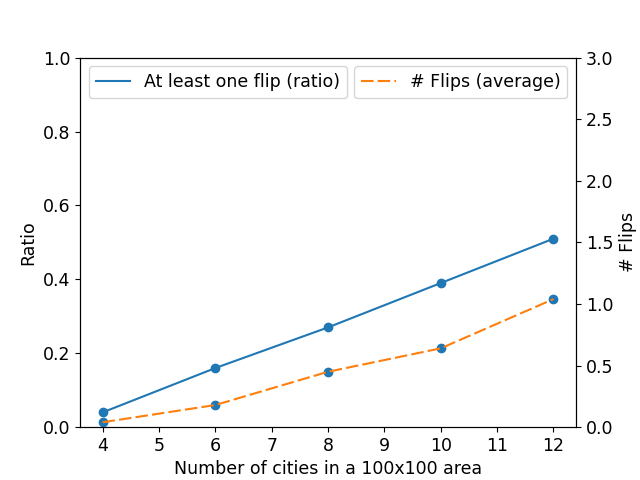
\includegraphics[width=5.14cm]{../figs/new_plot_n.png}
	\end{subfigure}
	~\hfill
	\begin{subfigure}[b]{0.32\textwidth}
		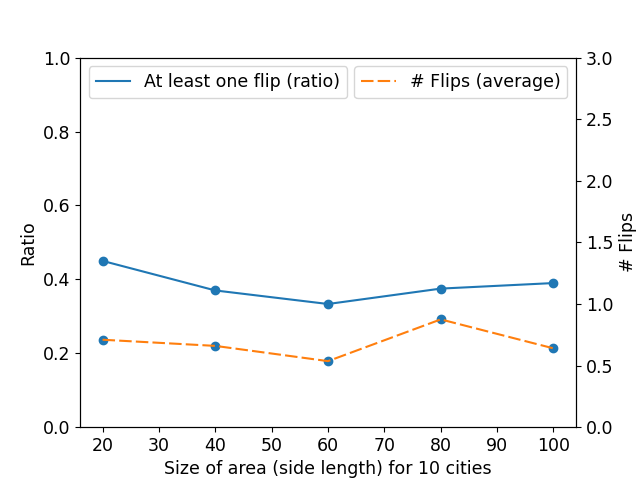
\includegraphics[width=5.14cm]{../figs/new_plot_space.png}
	\end{subfigure}
	~\hfill
	\begin{subfigure}[b]{0.32\textwidth}
		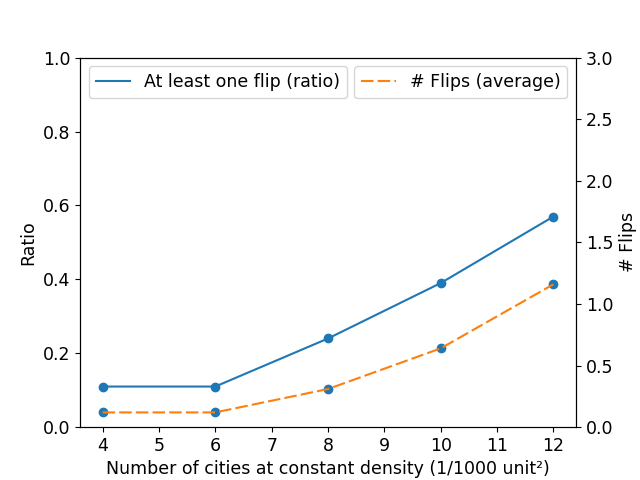
\includegraphics[width=5.14cm]{../figs/new_plot_both.png}
	\end{subfigure}
	\hspace{-3pt}
	%\vspace*{5pt}
	\caption{\small{\label{fig:experiments}Varying the number of cities (left), size of the area (middle), and both (right). The plots show the likelyhood of at least one flip and the average number of flips (over $100$ instances).}}
	%	\vspace*{-5pt}
\end{figure}

As a conclusion, we introduced a new version of \texttt{TSP}, in which controlling acceleration of a visiting vehicle plays a key role. We showed some preliminary results which already distinguish the problem from the well-known \texttt{Euclidean TSP}. We showed $NP$-completeness for the problem and presented multiple reductions. As algorithmic results, we proposed a heuristic using a combination of the flip heuristic with the $A^*$ algorithm. Finally, we presented some experimental results to validate said heuristic and quantify the difference between \texttt{ETSP} and \texttt{VTSP}.

%\nocite{*}
\bibliographystyle{alpha}
\bibliography{paper}
\label{sec:biblio}

\end{document}